%  -------------------------------------------------------------------------------
%  \author Jan P Buchmann <jan.buchmann@sydney.edu.au>
%  \copyright 2018 The University of Sydney
%  \description
%  -------------------------------------------------------------------------------
\usetikzlibrary{shapes.geometric, positioning, calc, shadings}
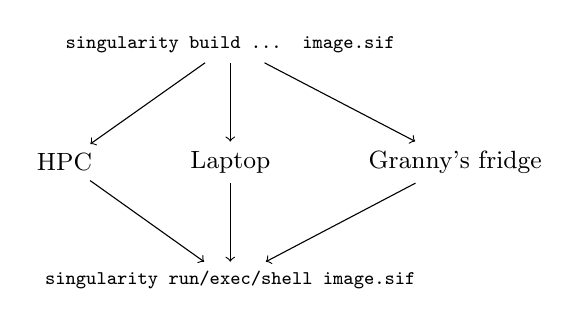
\begin{tikzpicture}[auto,font=\small,
                    every node/.style={node distance=1cm},
                    command/.style={rectangle, font=\scriptsize\ttfamily}]
    \def\blockdist{0.3}
    \node (container) [command]                        {singularity build ... image.sif};
    \node (laptop)    [below = of container]        {Laptop};
    \node (hpc)       [left = of laptop]        {HPC};
    \node (iot)       [right = of laptop]        {Granny's fridge};
     \node (image)    [command, below = of laptop] {singularity run/exec/shell image.sif};

    \path[->] (container) edge [] (laptop)
                          edge [] (hpc)
                          edge [] (iot);
    \path[->] (laptop)    edge [] (image)
              (hpc)       edge [] (image)
              (iot)       edge [] (image);
\end{tikzpicture}

% The comment style is used to describe the characteristics of each force
%comment/.style={rectangle, inner sep= 5pt, text width=4cm, node distance=0.25cm, font=\scriptsize\sffamily},
% The force style is used to draw the forces' name
%force/.style={rectangle, draw, fill=black!10, inner sep=5pt, text width=4cm, text badly centered, minimum height=1.2cm, font=\bfseries\footnotesize\sffamily}]
